\begin{anexosenv}

<<<<<<< HEAD
\chapter{Primeiro Anexo}

\begin{figure}[H]
    \centering
   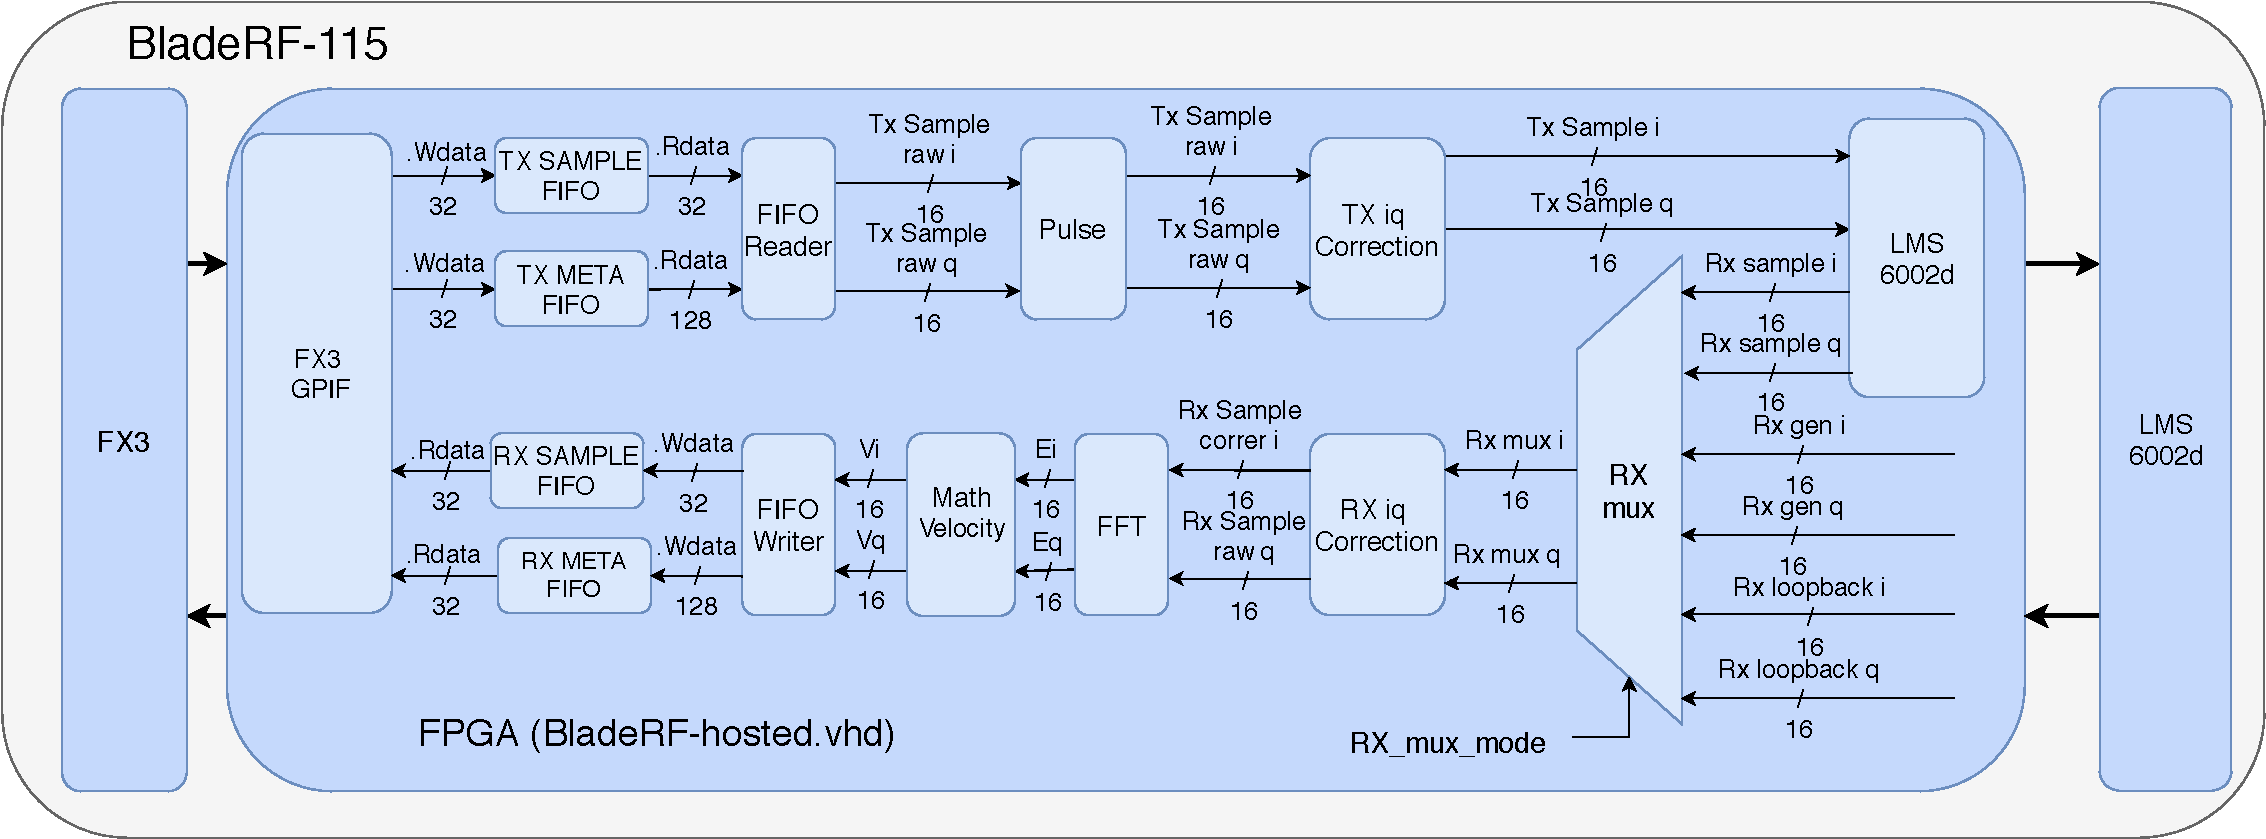
\includegraphics[scale = 0.58, angle=270]{arquitetura.pdf}
  \caption{Arquitetura desenvolvida para ser implementada em FPGA, sendo esta desenvolvida utilizando a ferramenta drawio.}
   \label{arquitetura1}
    \end{figure}
	
=======
\partanexos

\chapter{Primeiro Anexo}

\begin{figure}[H]
  \centering
  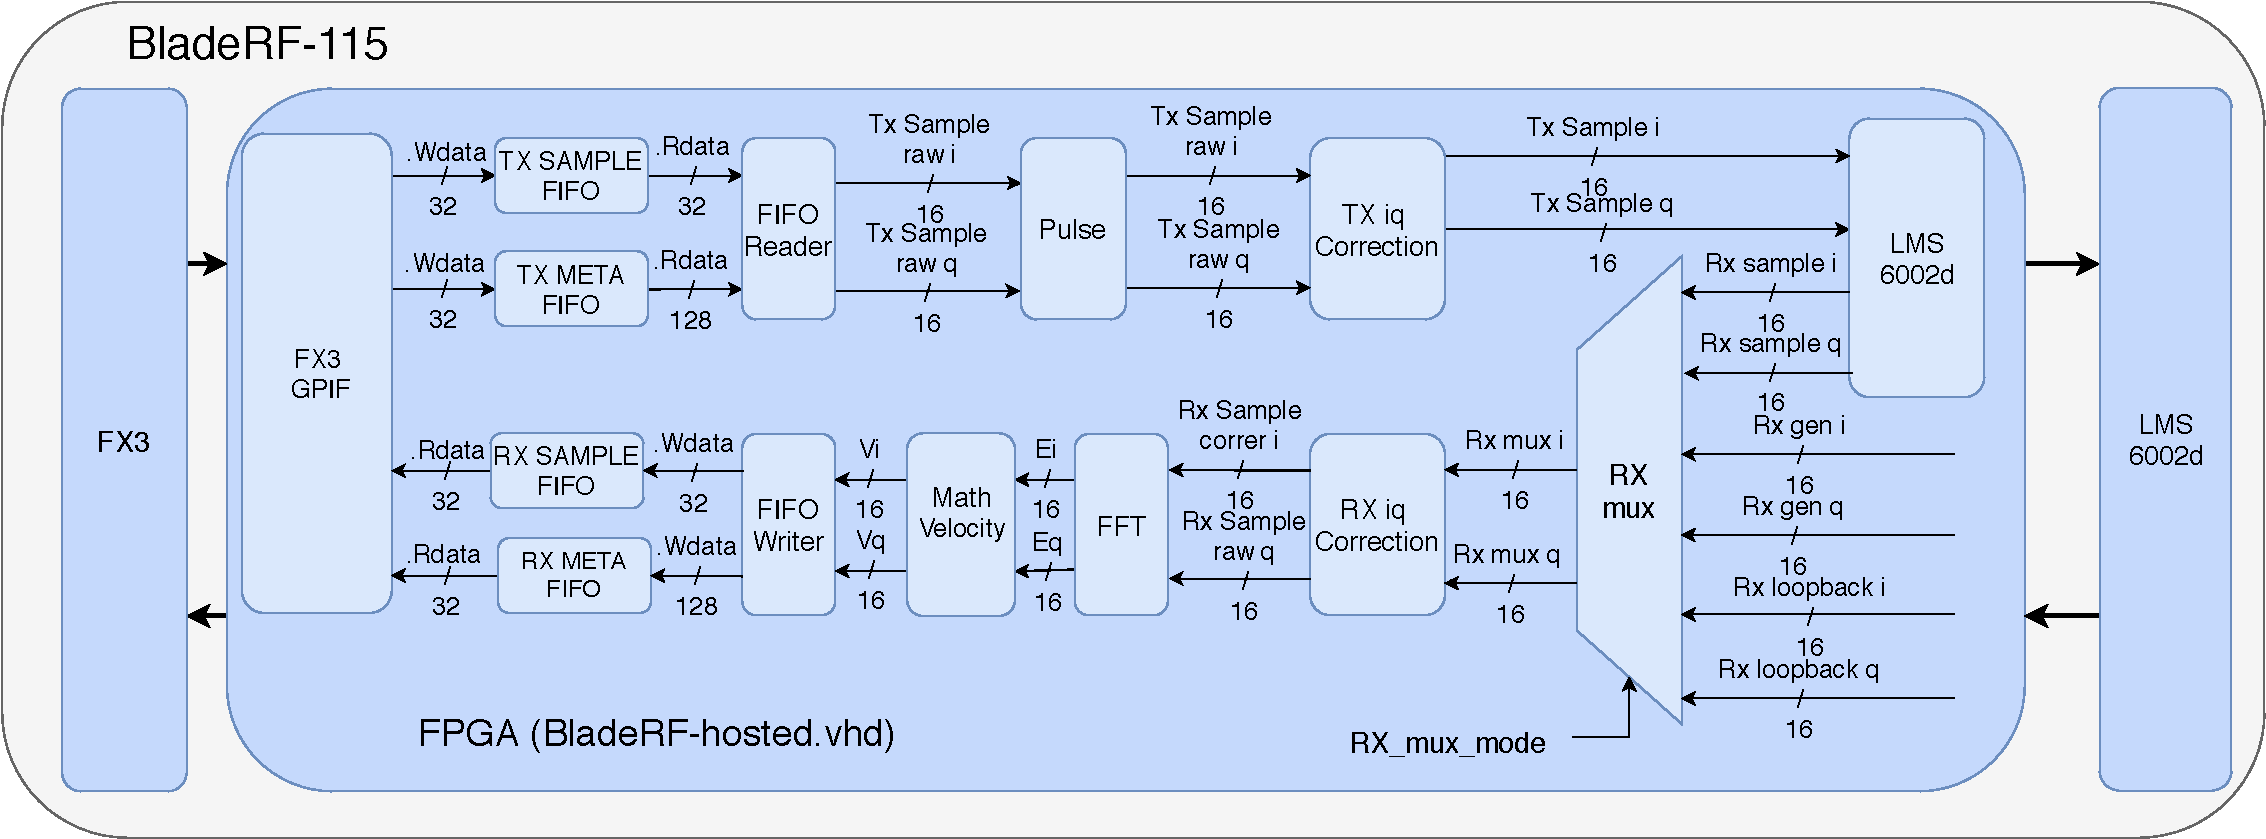
\includegraphics[scale = 0.58, angle=270]{arquitetura.pdf}
  \caption{Arquitetura utilizada pelo fabricante para emissão e recepção do sinal.}
  \label{arquitetura1}
\end{figure}
>>>>>>> 6b9454d3ddd256fae681e614507e68ec978b0c9d

\chapter{Códigos do MATLAB}
    
\chapter{Plantas dos Componentes}

\end{anexosenv}